\documentclass[../main.tex]{subfiles}
\graphicspath{{\subfix{../images/}}}
\begin{document}
\subsection*{Answers - Binomial expansion (page \pageref{Binomial Expansion})}
\label{Binomial expansion answers}

\begin{enumerate}
    \item \( (x+y)^3 = x^3 + 3x^2 y + 3xy^2 +y^3 \)
    \item 
    $
    \!
    \begin{aligned}[t]
     (2x+y)^4 
        &= (2x)^4 + 4(2x)^3y + 6(2x)^2y^2 + 4(2x)y^3 + y^4 \\
        &= 16x^4 + 32x^3y + 24x^2y^2 + 8xy^3 + y^4 \\
    \end{aligned}
    $ 
    \item 
    $
    \!
    \begin{aligned}[t]
     (2x-3)^5 
        &= (2x)^5 + 5(2x)^4(-3) + 10(2x)^3(-3)^2 + 10(2x)^2(-3)^3 + 5(2x)(-3)^4 + (-3)^5 \\
        &= 32x^5 -240x^4 +720x^3 - 1080x^2 + 810x - 243 \\
    \end{aligned}
    $

    \item 
    $
    \!
    \begin{aligned}[t]
     (3x+2y)^4 
        &= (3x)^4 + 4(3x)^3(2y) + 6(3x)^2(2y)^2 + 4(3x)(2y)^3 + (2y)^4 \\
        &= 81x^4 +216x^3y +216x^2y^2 + 96xy^3 + 16y^4 \\
    \end{aligned}
    $

    \item 
    $
    \!
    \begin{aligned}[t]
     (2x + \frac{1}{x^2} )^4 
        &= (2x)^4 + 4(2x)^3(\frac{1}{x^2}) + 6(2x)^2(\frac{1}{x^2})^2 + 4(2x)(\frac{1}{x^2})^3 + (\frac{1}{x^2})^4 \\
        &= 16x^4 + 32x + \frac{24}{x^2} + \frac{8}{x^5} + \frac{1}{x^8}\\
    \end{aligned}
    $
    
    \item We need to find when the powers in a term cancel out and leave a constant. \\
    \((3x^2)^m(\frac{-1}{3x})^n\) \\
    We can form two equations from this: \\
    \( \frac{x^{2m}}{x^n} = x^0 \)\\
    \( 2m - n = 0 \)\\
    And we know in this question that \( m + n = 12\) \\
    Solving, we get \(m=4, n=8 \).\\
    This means that if we look in row 12, we look for the column where \( m=4 \) to get the coefficient.\\
    \begin{figure}[h]
        \centering
        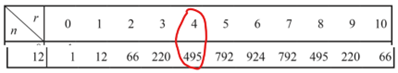
\includegraphics[width=0.5\linewidth]{images/Picture2.png}
    \end{figure}
    Therefore, our term is \( 495(3x)^4(\frac{-1}{3x})^8 = \frac{495}{81} = \frac{55}{9}\)
    
    \item We need to find when the powers in a term cancel out to give \(x^2\)\\
    Forming two equations from \( (x^2)^m(\frac{1}{x})^n\)\\
    \( \frac{x^{2m}}{x^n}=x^2 \xrightarrow{}2m-n=2\)\\
    Also, \(m+n=10\)\\
    Solving, we get \(m=4, n=6\)\\
    From row 10, we see that when \( m=4 \), the coefficient is 210.\\
    \begin{figure}[h]
        \centering
        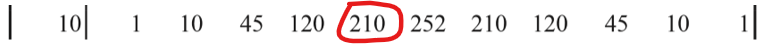
\includegraphics[width=0.5\linewidth]{images/Picture3.png}
    \end{figure}
    Therefore, our term is \( 210(x^2)^4(\frac{1}{x})^6=210x^2\)

    \item Forming two equations from \( (2x^2)^m(\frac{-3}{x})^n\)\\
    \( \frac{x^2m}{x^n}=x^0 \xrightarrow{}2m-n=0\)//
    Also, \( m+n=6\)\\
    Solving, we get \(m=2, n=4\)\\
    From row 6 we see that when \(m=2\), the coefficient is 15.\\
    Therefore our term is \( 15(2x^2)^2(\frac{-3}{x})^4=15*4*81=4860\)
    \begin{figure}[h]
        \centering
        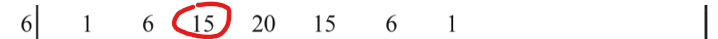
\includegraphics{images/Picture4.png}
    \end{figure}

    \item
    $
    \!
    \begin{aligned}[t]
     \cos^6(\theta)
        &=(\frac{e^{i\theta}+e^{-i\theta}}{2})^6= (\frac{1}{2})^6(e^{i\theta}+e^{-i\theta})^6 \\
        &= \frac{1}{64}(e^{6i\theta}+6(e^{5i\theta})(e^{-i\theta})+15(e^{4i\theta})(e^{-2i\theta})+20(e^{3i\theta})(e^{-3i\theta})+15(e^{2i\theta})(e^{-4i\theta})\\
        &+6(e^{i\theta})(e^{-5i\theta})+e^{-i\theta})\\
        &=\frac{1}{64}(e^{i\theta}+e^{-i\theta}+6e^{4i\theta}+6e^{-4i\theta}+15e^{2i\theta}+15e^{-2i\theta}+20)\\
        &=\frac{1}{32}[(\frac{e^{6i\theta}+e^{-6i\theta}}{2})+6(\frac{e^{4i\theta}+e^{-4i\theta}}{2})+15(\frac{e^{2i\theta}+e^{-2i\theta}}{2})+\frac{20}{2}]\\
        &=\frac{1}{32}\cos(6\theta)+\frac{3}{16}\cos(4\theta)+\frac{15}{32}\cos(2\theta)+\frac{5}{16} \text{(As required)}
    \end{aligned}
    $
    
\end{enumerate}
\end{document}